\subsection{空对象模式}

空对象模式(Null Object pattern)是一种设计模式,它的主要目的是在处理空值的情况时,避免出现空指针异常。

在空对象模式中,当遇到空值时,会返回一个特殊的空对象,这个空对象实现了与原对象相同的接口,但是它不会执行任何实际的操作。这样,程序在调用空对象的方法时,不会抛出空指针异常,而是会返回默认的结果。

使用空对象模式的主要目的是提高程序的健壮性和可维护性。它可以帮助开发人员避免在处理空值时出现空指针异常,从而使程序更容易维护和扩展。

空对象模式通常用于处理复杂的数据结构,例如树形结构或链表结构。在这些数据结构中,空值是很常见的,如果不使用空对象模式处理这些空值,程序很容易出现空指针异常。

\begin{figure}[htb]
  \centering
  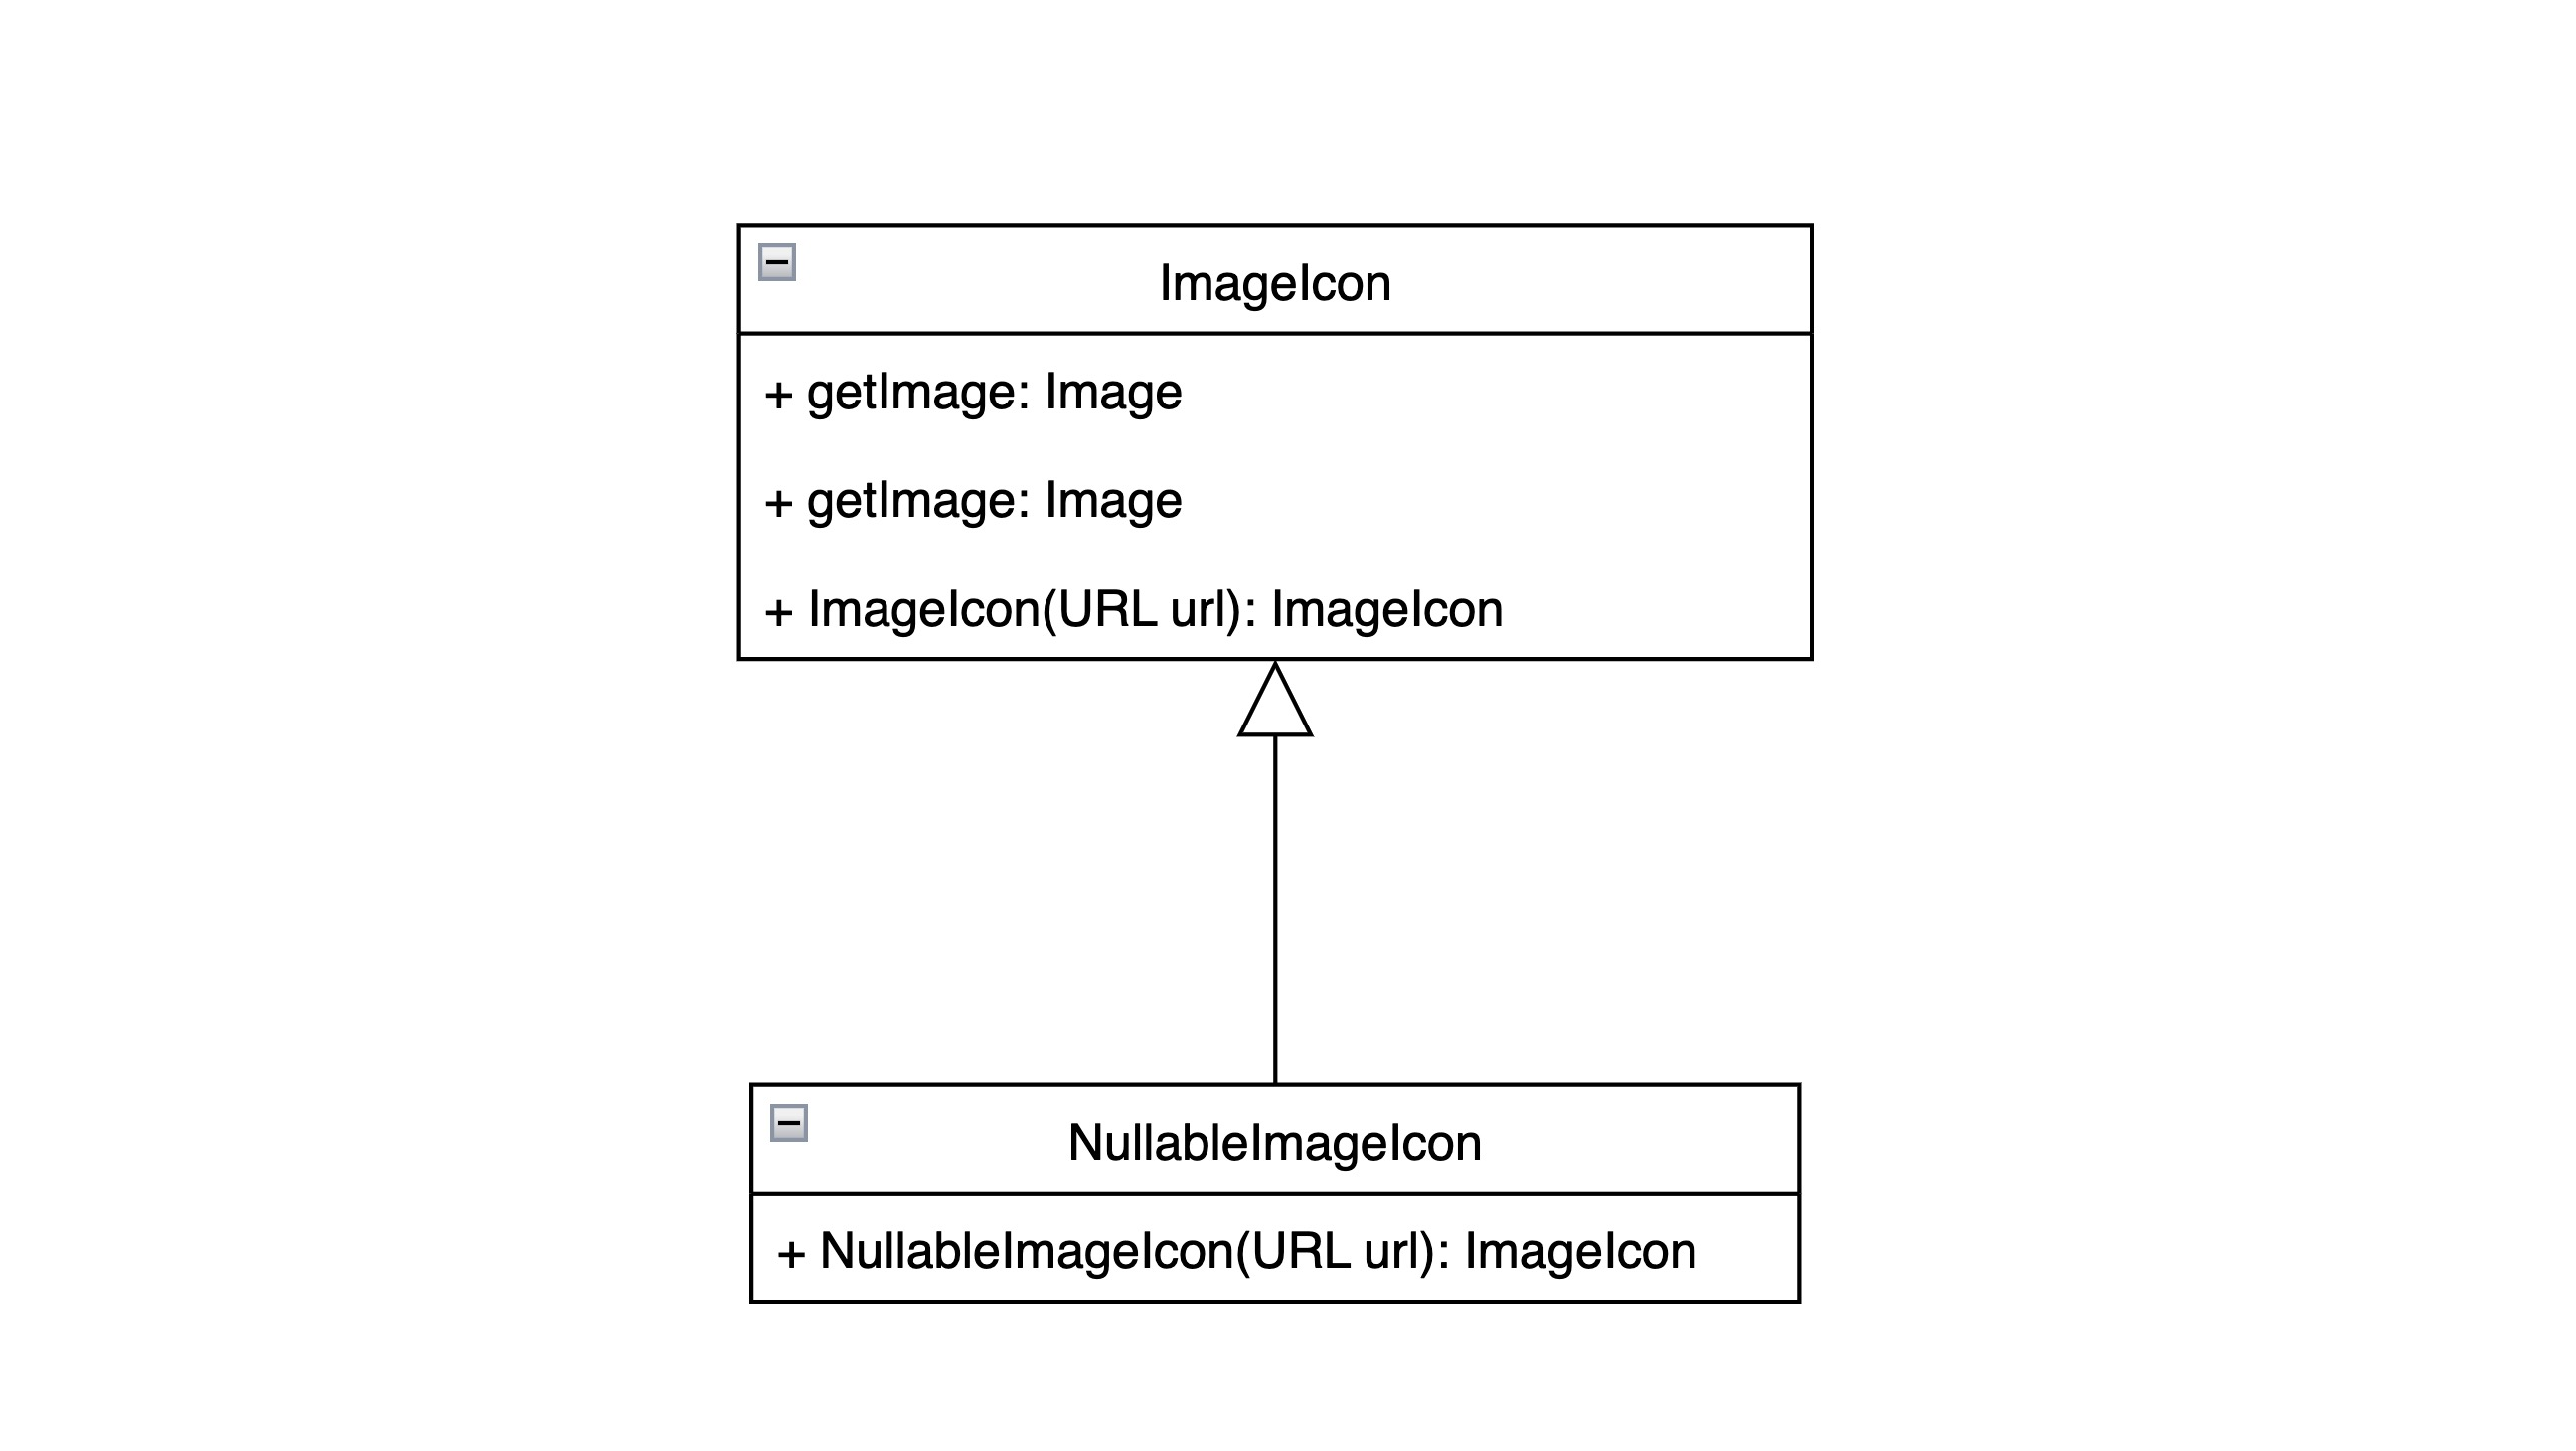
\includegraphics[width=0.9\textwidth]{figures/空对象模式.jpg}
  \caption{空对象模式在 Slow6502 中的类图}
\end{figure}

在StatusPanel组件中使用空对象模式,使得即使在没有资源文件图片存在的情况下,也可以正常显示图片组件,以默认图片作为空对象。

